\chapter{Criptosistemas clásicos}

La criptografía tiene como objetivo resolver el siguiente problema:

\begin{figure}[h]
	\begin{center}
		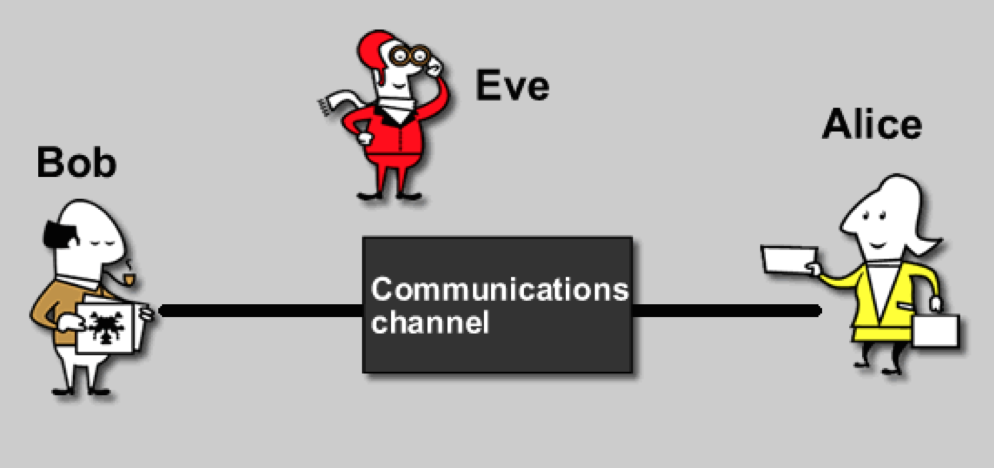
\includegraphics[width=0.5\textwidth]{img/aliceBobEve.png}
		\caption{Cómo enviar un mensaje de manera segura entre Bob y Alice por un canal al que Eve tiene acceso}
	\end{center}
\end{figure}


El objetivo es garantizar tanto la confidencialidad del mensaje (Eve no es capaz de saber qué se están diciendo) como de autentifiación (Alice está segura de que es Bob quien mandó el mensaje y viceversa)

A lo largo de este capítulo veremos los métodos que han sido empleados a lo largo de la historia para lograr este objetivo.

	\section{Esteganografía}

		Intentar ocultar la existencia del mensaje. Es un método con origen muy antigüo (~486-425 a.C)

	\section{Criptografía}
		\begin{defn}[Criptografía]
		Tradicionalmente se ha definido como el ámbito de la criptología el que se ocupa de las técnicas de cifrado o codificado destinadas a alterar las representaciones lingüísticas de ciertos mensajes con el fin de hacerlos ininteligibles a receptores no autorizados.

		El primer método de criptografía data del siglo V antes de cristo
		\end{defn}

		La mayoría de estos métodos se basaban en transposición.

		\begin{defn}[Transposición]
			Cambio en el orden de las letras de un mensaje
		\end{defn}

		\subsection{El criptosistema de Cesar}

			Se utiliza la sustitución como método de encriptación, normalmente cambiando cada letra por su correspondiente al desplazarse $d$ espacios atrás en el abecedario. Por ejemplo:
			\begin{center}
			\begin{tabular}[h]{c|c}
			sin cifrar & cifrado \\ \hline
			A & D\\
			B & E\\
			C & F\\
			... & ...
			\end{tabular}
			\end{center}

		\subsection{Formalización}

		Vamos a ver cómo denominamos formalmente los elementos que intervienen en un proceso de cifrado:
		\begin{itemize}
			\item \textbf{Mensajes}

			Tenemos dos diferentes mensajes en todo proceso de cifrado
			\begin{enumerate}
			\item M = Mensajes en claro
			\item C = Mensajes cifrados
		\end{enumerate}

		\item \textbf{Alfabeto}
		Tendremos un alfabeto o dos, dependiendo de si los alfabetos de M y C son el mismo o no.

		Ejemplos de alfabetos serían:
		\begin{itemize}
			\item $A = \{A,B...Z\}$
			\item $A = \{0,1\}$
			\item $A = \{A,B...Z,\hdots,\text{?`},\text{?},1,2,3,\hdots,9,0\}$
			\item $A = $ Código ASCII
		\end{itemize}

		\item \textbf{Funciones para cifrar}

		Serán funciones de la forma $f: M \rightarrow C$ donde $f$ es inyectiva

		\item \textbf{Funciones para descifrar}

		Serán funciones de la forma $f^{-1}: C \rightarrow M$ donde $f$ es la misma función empleada para cifrar el mensaje.
		\end{itemize}

		Para que pueda llevarse a cabo la comunicación entre $A$ y $B$, A debe conocer $f$ y $B$ debe conocer $f^{-1}$. A envía un mensaje $m\in M$ a $B$ usando $f(m)=c$ y enviando $c$. $B$ puede obtener el mensaje calculando $f^{-1}(c) = m$.

		En este modelo, romper el sistema de cifrado equivale a que un tercero averigüe $f^{-1}$.


		\textbf{¿Podemos usar más de una función para cifrar?}

		En el sistema de Cesar se puede cambiar, por ejemplo, la longitud desplazmiento por el abecedario al realizar la encriptación, aunque no hay muchas posibilidades.

		\begin{defn}[Criptosistema]
			Colección de functiones para cifrar:

			$f_e : M_e \rightarrow C_e$

		\end{defn}


		\vspace{1.5cm}

		\begin{example}{Como romper la criptografía Cesar}

			Se puede romper "facilmente" la criptografía Cesar con análisis de frecuencias. Por ejemplo, en castellano la letra más frecuente es la E, con un 13,68\%, sabiendo la letra más frecuente de un mensaje cifrado se puede calcular la distancia entre esa y la E y muy probablemente hayamos hallado la clave de cifrado.

			La fiabilidad de este método puede verse mermada por la genericidad del texto cifrado. Si es corto y si habla de un tema en particular es posible que las frecuencias varíen respecto a otros textos genéricos en Español.

			De hecho, por ejemplo, en el manual de UNIX la frecuencia de la letra e baja al 9\% dejando a la letra relegada al cuarto puesto, por detrás de la t, la n y la i.

		\end{example}


		Veamos la frecuencia general de distintos grupos de letras en ingles.

		\begin{tabular}[h]{r|c|c}
			\textbf{grupos} & \textbf{frec} & \textbf{rango} \\ \hline
			e & 12.7\% & 12.7 \\
			taoiushr & 56.9 & 6-9 \\
			cumwfgypb & 19.9 & 1.5 - 3 \\
			vkjxqz & 2.2 & < 1
		\end{tabular}

		\section{Criptosistema afín (sobre letras)}

			\begin{defn}[Cifrado afín]
			El cifrado afín también se le llama cifrado de transformación afín o cifrado monoalfabético genérico. Es un tipo de cifrado por sustitución en el que cada símbolo del alfabeto en claro (el alfabeto del texto en claro) es sustituido por un símbolo del alfabeto cifrado (el alfabeto del texto cifrado) siendo el número de símbolos del alfabeto en claro igual que el número de símbolos del alfabeto cifrado. Para hallar el símbolo del alfabeto cifrado que sustituye a un determinado símbolo del alfabeto en claro, se usa una función matemática afín en aritmética modular. Para poder aplicar la función matemática lo primero que hay que hacer es asignar un orden que a cada símbolo de cada uno de los alfabeto le asocie un número de orden.
			\end{defn}

			Si tenemos un alfabeto de N letras $\leftrightarrow \mathbb{Z}/N$ y denominamos a las claves: $a,b \in \mathbb{Z}/N$, tenemos que el proceso de cifrado puede representarse mediante la siguiente fórmula matemática:

			\begin{align*}
				f_{a,b} :&  \mathbb{Z}/N\to \mathbb{Z}/N\\
				& x \rightarrow ax + b
			\end{align*}

			\subsection{¿Para qué valores de a,b es $f_{a,b}$ inyectiva?}

			Para verlo calculamos $f^{-1}_{a,b}$

			$$ax+b = y$$
			$$ax = y - b$$

			Si $a \in U(\mathbb{Z}/N)
			\implies
			x = a^{-1} (y-b) \implies
			x = a^{-1}y - a^{-1}b$


			$$f^{-1}_{a,b} = f_{a^{-1},-a^{-1}b}$$

			Así hemos demostrado que:

			\begin{enumerate}
				\item $a \in U(\mathbb{Z}/N) \Rightarrow f_{a,b}$ inyectiva
				\item En ese caso si $e = (a,b)$ es la clave para cifrar $\Rightarrow d = (a^{-1},-a^{-1}b)$ es la clave para descifrar.
			\end{enumerate}

			Usando la definición de inyectiva:

				$$ \exists \alpha \in q : a \alpha = 1 \Leftrightarrow a \alpha + b = 1 + b $$

			Así llegamos a la conclusión de que en realidad el par $(a,b)$ tiene ciertas restricciones:

			$$ E = \{ (a,b): a \in U(\mathbb{Z}/N), b \in \mathbb{Z}/N \} $$

			$$ \#E = \#U(\mathbb{Z}/N) * \#\mathbb{Z}/N $$


			\begin{prop}
				Sea $a \in \mathbb{Z}/N : a \in U(\mathbb{Z}/N) \Leftrightarrow (a,N) = 1$ (son primos entre si).

				\begin{proof}

					\textbf{$\Rightarrow$}

					$$\exists \alpha \in \mathbb{Z}/N : a \alpha \equiv 1 \mod n \Rightarrow \exists k : a\alpha + kN = 1$$

					$$\text{Si } (a,N) \neq 1 \Rightarrow \exists p \text{ primo } : p | a, N \Rightarrow p | ax + 1 (FALTA UN PELÍN)$$

					\textbf{$\Leftarrow$}

					$(a,n) = 1$. Esto se demuestra usando el algoritmo de euclides.

				\end{proof}
			\end{prop}


			Volvemos entonces al número de claves ya que sabemos como calcularlo:

			$$ \#E = \#U(\mathbb{Z}/N) * \#\mathbb{Z}/N = \phi(N)*N $$


			\subsection{La función de Euler}

				\begin{defn}[Función de Euler]
				La función φ de Euler (también llamada función indicatriz de Euler) es una función importante en teoría de números. Si n es un número entero positivo, entonces φ(n) se define como el número de enteros positivos menores o iguales a n y coprimos con n, es decir, formalmente se puede definir como:

				\[\phi(m) = \left| \{n \in \nat \tq n \leq m \wedge mcd(m,n)=1\}\right|\]

				En el caso de que queramos calcular la función de Euler de un número primo $p$ tenemos:

				$\phi(p) = p-1$

				$\phi(p^n) = p^{n} - p^{n-1} = p^{n-1} p(p-1) = p^{n}(1- \frac{1}{p})$

				Como es una función multiplicativa:

				$\phi(N) =N \Pi \phi(P_i^{n_i}) = \Pi P_i^{n_i} n_i \Pi (1- \frac{1}{p_i}) = N \Pi(1 - \frac{1}{p_i})$

				\end{defn}

\begin{figure}[h]
	\begin{center}
		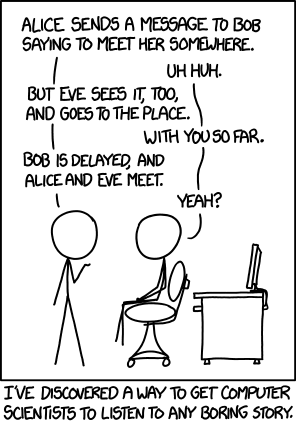
\includegraphics[width=0.5\textwidth]{img/protocol.png}
	\end{center}
\end{figure}

Veamos un ejemplo de como un espía podría realizar un ataque contra un usuario que emplea este sistema de cifrado.
\begin{example}
El objetivo es conseguir conocer los valores $a$ y $b$ que han sido empleados para lo que deberemos resolver un sistema de dos ecuaciones de dos incógnitas, una vez hemos obtenido una muestra de un texto cifrado y su original sin cifrar.

Como, en teoría, el atacante no tendría acceso al texto original, empleará una tabla de frecuencias que, en un texto en inglés, nos dice que las letras más frecuentes son la E y la T.

Ahora podemos estudiar el texto cifrado y ver que las letras más usadas son, respectivamente, U y D. Por tanto, convirtiendo estas letras en sus correspondientes números (según la posición que ocupan en el alfabeto inglés) tenemos el siguiente sistema de ecuaciones:
\[
\left\{
20α + β = 4\atop
2α +β = 19
\right.\]

Que, si restamos a la primera ecuación la segunda y nos apoyamos en el hecho de que estamos trabajando en $\ent_{26}$ nos queda:
\[
\left\{
20α + β = 4\atop
17α = 11
\right.\]

Ahora debemos encontrar el inverso multiplicativo de 17 trabajando en módulo 26, para lo que emplearemos el algoritmo de Euclides.

\begin{enumerate}
\item $26 = 17 + 9$
\item $17 = 9 + 8$
\item $9 = 8 + 1 $
\item $8 = 8 \cdot 1 + 0$
\end{enumerate}

Como al final hemos obtenido un $+0$ el propio algoritmo de Euclides nos garantiza que existe el inverso multiplicativo modulo 27 de 17.

Ahora aplicamos el algoritmo de Euclides para obtener el inverso y para ello expresamos cada resto sustituyendo en la fórmula resultando el resto siguiente. Es decir:
\[1 = 9 - 8 = 9- (17-9) = 2 \cdot 9 - 17 = 2 \cdot (26 - 17) - 17 = 2 \cdot 26 - 3 \cdot 17 = -24 \cdot 26 + 23 \cdot 17 \implies \]
\[\implies 1 + 24 \cdot 26 = 23 \cdot 17 \implies 1 = 23 \cdot 17\]
Con ello llegamos a que:
\[\frac{1}{17} = 23 \implies α = 23 \cdot 11 = 19 \& β = 14\]
\end{example}

Veamos otro ejemplo un poco más interesante.
\begin{example}
En este caso consideramos que el conjunto de símbolos válidos empleados por el emisor al escribir el texto original son: el alfabeto inglés, el espacio y el símbolo de interrogación.

En este caso el espía intercepta un mensaje y encuentra que los símbolos más habituales en ese mensaje han sido la B y ?. En este caso no podemos emplear la misma tabla de frecuencias que en el ejemplo anterior, puesto que el alfabeto inicial ha cambiado.

Con las nuevas condiciones tenemos que las letras más habituales se relacionan de la forma:
\[B \to \_ \]
\[? \to E\]
que nos lleva al sistema de ecuaciones:
\[
\left\{
α+β = -2\atop
-α+β = 4
\right. \implies 2α = -6\]

Pero en esta ocasión no podemos emplear el algoritmo de Euclides, pues el 2 no es coprimo con 6 ni con su inverso aditivo.

En esta ocasión, el problema se debe a que estamos trabajando en $\ent_{28}$ que es un cuerpo con divisores de 0 y, por tanto, el sistema de ecuaciones no tendrá una única solución sino varias. En este caso nos quedan que son soluciones posibles los pares de valores:
\[α=11, \ β=15 \;\;\; \& α=25 \ β=1\]

Ahora lo que podríamos hacer es probar ambas combinaciones y ver cuál de ellas nos permite obtener un texto original con sentido.

Otra posibilidad es acudir a la tabla de frecuencias y ver cuál de los dos sistemas nos permite obtener la siguiente letra más frecuente. Si las cosas funcionan bien, sólo uno de los dos sitemas nos funcionará.

Así, tomamos la I, que es la tercera letra más habitual en el mensaje cifrado y vemos que nuestros valores de α y β nos llevan a que la letra original podría ser T o F.

Puesto que la T es una de las letras menos habituales, la hipótesis razonable es pensar que los valores correctos de α y β es $(11,15)$.
\end{example}

Tras estos ejemplos hay una duda que debería surgir directamente en el lector. En ambos ejemplos nos hemos basado en un absoluto conocimiento acerca del sisteme alfanumérico empleado en el mensaje original, pero esto no es realista.

Para explicar esto debemos fijarnos en el \textbf{Principio de Kerkhoffs} que dice:
\begin{prop}[Principio de Kerkhoffs]
No puede requerirse que un criptosistema sea secreto. Tiene que poder caer en manos del enemigo sin que esto suponga un inconveniente.

Es decir: la seguridad del sistema tiene que depender UNICAMENTE de mantener secretas las claves.
\end{prop}

Recordemos que el sistema de Cesar tenía el gran inconveniente de que había muy pocas posibilidades. Es decir, con hacer 26 pruebas se puede obtener el mensaje original a partir de un mensaje cifrado.

Este problema se ha relajado mediante el empleo de la criptografía afín pero, como acabamos de ver, sigue siendo sencillo descifrar un mensaje.

Con el fin de mejorar la seguridad aparece el \textbf{Criptosistema de sustitución}

\section{Criptosistema de sustitución}

Este sistema simplemente consiste en una mejora del sistema César. En lugar de desplazar todas las letras del alfabeto lo que se hace es tomar una reordenación del mismo.

% TRASPAS
\section{Definción de Criptabeto}

El problema de los sistemas que hemos visto, y sobre todo del último, es que es necesario que el emisor y el receptor del mensaje se pongan de acuerdo en la relación alfabeto original - alfabeto crifrado que se va a emplear.

Para llevarlo a cabo existen diferentes alternativas:
\begin{itemize}
\item \textbf{Frase clave}

\item \textbf{Palabra clave - lectura clave}
\end{itemize}